\chapter{Evaluation}
\label{chap:evaluation}
\section{Example Models and Case Study}
\subsection{Different Constraint Types and their Handling}
\label{sec:evaluationAcademicModels}
Every of the following problem types can have only floating point variables or be a mixed-integer problem
Many solvers have the ability to solve a given problem also as mixed integer problem. For the pure constraint satisfaction this should be no problem. But i will become a problem, when also a boundary Value is demanded.
\subsubsection{Linear}
\paragraph{Pure Floating Point Variables}
\paragraph{Mixed Integer}
solve with cplex up to 100000 Variables possible
\subsubsection{Non linear convex}
solvable with every Solver implementing some version of Newton Algorithm on Sparse Matrices like Minos, Knitro or Quadratic programming approaches like in CPLEX.
\subsubsection{Non Convex}
\label{sec:exampleModelNonConvex}
\begin{figure}
\label{fig:pumpTyre}
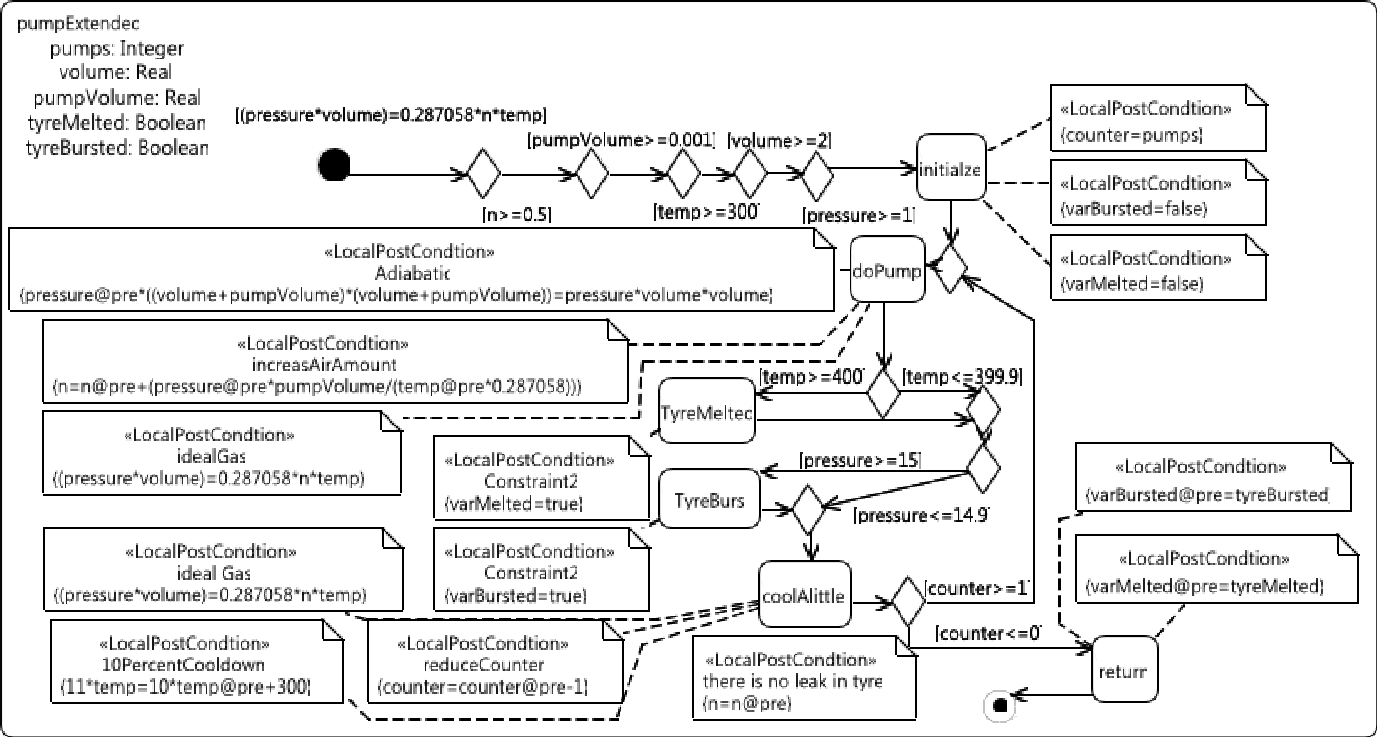
\includegraphics[width=\textwidth]{./pics/pumpTyre.pdf}
\caption{Activity Diagram with non convex mixed integer constraints}
\end{figure}
in general undecidable couenne finds solutions sometimes.
The Example Model here is the Exploding Tyre Model
\subsubsection{Constraint Programming}
ILOGCP, Gecode or transformation possible
\paragraph{Integer arithmetic only} Gecode
\paragraph{linear mixed Integer arithmetic} IlogCP
\begin{figure}
\label{fig:classifyTriangle}
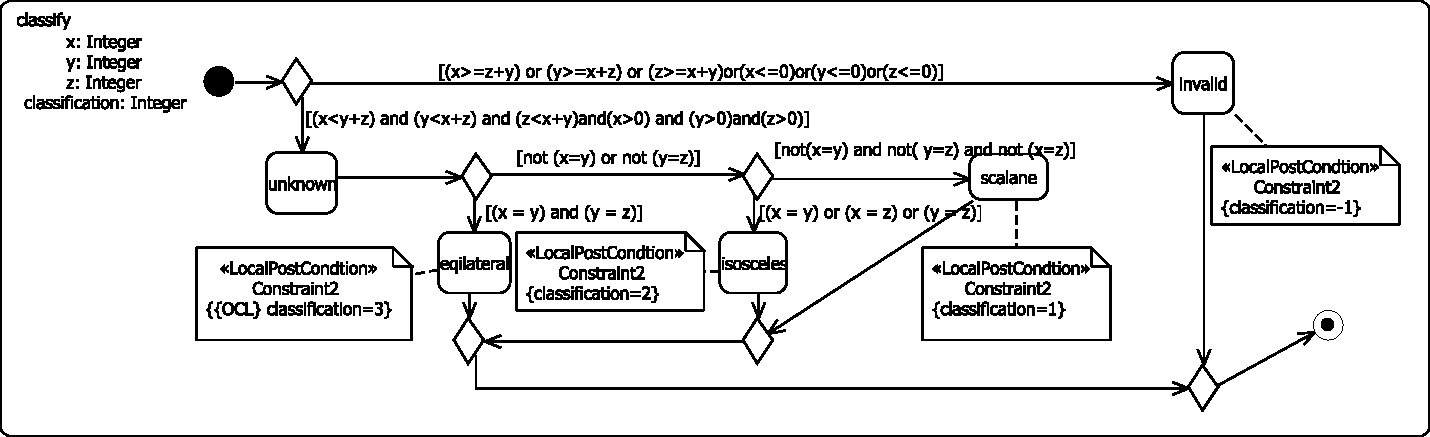
\includegraphics[width=\textwidth]{./pics/TriangleClassificator.pdf}
\caption{Activity Diagram with non convex mixed integer constraints}
\end{figure}
\paragraph{nonlinear mixed Integer arithmetic}
really really really problematic. Currently the only way is to transform the Activity Test Case Graph to remove the Logical Operations in favour of parallel or sequential Control Flows with guards. Use COUENNE.
\subsection{Case Study PAX Model}
\label{sec:evaluationCaseStudy}
I could do a case study with the Airbus PAX call model from Atego.
\section{Limitations}
\label{sec:evaluationLimitations}
\subsection{Theoretical Limitations}
undecidability of nonlinear arithmetic over infite sets and Exponential runtime for Constraint solving algorithms for some formulations
\subsection{Limitations of the Implementation}
no structured activity nodes, no invariants, not completely implemented test goal management.
\subsection{Limitations of used Tools}
XMI interchange format does not work always LOTS OF BUGS!!!!
\subsubsection{AMPL}
\label{sec:LimitationsAMPL}
\section{further Ideas}
There is no good reason for using OCL as the specification language in order to ease the constraint solving prolog could directly be used as language to specify constraints in a UML Model.


